\documentclass{standalone}
\usepackage{mathpazo}
\usepackage{tikz}
\usetikzlibrary{calc}

\begin{document}
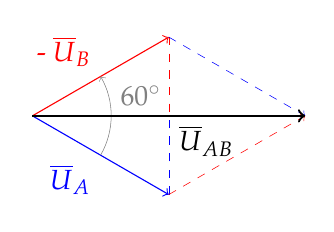
\begin{tikzpicture}
  \draw (0,0) coordinate (N);
  \draw (-30:2) coordinate (A);
  \draw (30:2) coordinate (B);
  \draw ($2*sqrt(3)*(1,0)$) coordinate (S);
  \draw[->, color = blue] (N) -- (A) node[below left, midway] {$\overline{U}_A$};
  \draw[->, color = red] (N) -- (B) node[above left, midway] {- $\overline{U}_B$};
  \draw[->, color = gray, very thin] (-30:1) arc[start angle = -30, end angle = 30, radius = 1cm] node[midway, above right] {$60^\circ$};
  \draw[-, color = blue, dashed, very thin] (A) -- ($(A)!(N)!(B)$);
  \draw[-, color = red, dashed, very thin] (B) -- ($(A)!(N)!(B)$);
  \draw[->, color = red, very thin, dashed] (A) -- (S);
  \draw[->, color = blue, very thin, dashed] (B) -- (S);
  \draw[->, thick] (N) -- (S) node[below right, midway] {$\overline{U}_{AB}$};
  \end{tikzpicture}
\end{document}